\documentclass[aspectratio=169]{beamer}
\mode<presentation>
{
  \usetheme{metropolis}      % or try Darmstadt, Madrid, Warsaw, ...
  \usecolortheme{default} % or try albatross, beaver, crane, ...
  \usefonttheme{structurebold}  % or try serif, structurebold, ...
  \setbeamercolor{background canvas}{bg=white}
  \setbeamertemplate{navigation symbols}{}
  \setbeamertemplate{bibliography item}{\insertbiblabel}
  %\setbeamertemplate{caption}[numbered]
} 

\setbeamertemplate{caption}{\raggedright\insertcaption\par}

\usepackage[english]{babel}
\usepackage[utf8x]{inputenc}
\usepackage{listings}             % Include the listings-package
\hypersetup{
    colorlinks = true,
    linkcolor = {black},
    urlcolor = {blue}
}
\usepackage{animate}

\DeclareMathOperator*{\argmin}{arg\,min}

\title[Deep Learning and Temporal Data Processing]{Deep Learning and Temporal Data Processing}
\subtitle{2 - Convolutional Neural Networks}
\institute{University of Modena and Reggio Emilia}
\author{Andrea Palazzi}
%\date{June 21th, 2017}

\def\thisframelogos{}

\newcommand{\framelogo}[1]{\def\thisframelogos{#1}}

\addtobeamertemplate{frametitle}{}{%
\begin{tikzpicture}[remember picture,overlay]
\node[anchor=north east] at (current page.north east) {%
    \foreach \img in \thisframelogos {%
        %\hspace{.5ex}%
        \includegraphics[height=3.5ex]{\img}%
    }%
};
\end{tikzpicture}}

\begin{document}

\framelogo{img/template/logo_unimore_white.png}

\bgroup
\renewcommand{\insertframenumber}{}
\begin{frame}[noframenumbering]
  \titlepage
\end{frame}
\egroup
\begin{frame}{Agenda}
  \tableofcontents
\end{frame}



%%%%%%%%%%%%%%%%%%%%%%%%%%%%%%%%%%%%%%%%%%%%%%%%%%%%%%%%%%%%%%%%%%
%%%%%%%%%%%%%%%%%%%%%%%%%%%%%%%%%%%%%%%%%%%%%%%%%%%%%%%%%%%%%%%%%%
%%%%%%%%%%%%%%%%%%%%%%%%%%%%%%%%%%%%%%%%%%%%%%%%%%%%%%%%%%%%%%%%%%


\section{Introduction}

%%%%%%%%%%%%%%%%%%%%%%%%%%%%%%%%%%%%%%%%%%%%%%%%%%%%%%%%%%%%%%%%%%

\begin{frame}{CNNs: overview}
Convolutional Neural Networks are very similar to ordinary Neural Networks.\\
\begin{itemize}
\item They are made up of neurons that have learnable weights and biases.
\item Each neuron receives some inputs, performs a dot product and optionally follows it with a non-linearity.
\item The whole network still expresses a single differentiable function.
\end{itemize}
\end{frame}

%%%%%%%%%%%%%%%%%%%%%%%%%%%%%%%%%%%%%%%%%%%%%%%%%%%%%%%%%%%%%%%%%%

\begin{frame}{CNNs: overview}
However, \textbf{CNNs make the explicit assumption that inputs are images}.
\begin{itemize}
\item \large{This architecture constraint paves the way to more efficient implementation, better performance and a vastly reduced amount of learnable parameters \emph{w.r.t.} fully-connected deep networks.}
\end{itemize}
Most important peculiarities of CNNs are presented in the following slides.
\end{frame}


%%%%%%%%%%%%%%%%%%%%%%%%%%%%%%%%%%%%%%%%%%%%%%%%%%%%%%%%%%%%%%%%%%
%%%%%%%%%%%%%%%%%%%%%%%%%%%%%%%%%%%%%%%%%%%%%%%%%%%%%%%%%%%%%%%%%%
%%%%%%%%%%%%%%%%%%%%%%%%%%%%%%%%%%%%%%%%%%%%%%%%%%%%%%%%%%%%%%%%%%


\section{Architecture}

\begin{frame}{CNN Architecture}
Unlike a regular neural network, CNN layers have neurons arranged in 3 dimensions: width ($W$), height ($H$) and depth ($C$).
\begin{figure}
\begin{tabular}{c}
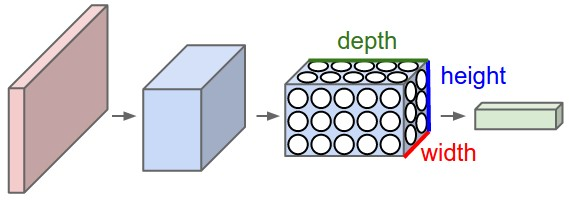
\includegraphics[width=0.5\textwidth]{img/cnn/cnn_vs_dnn.jpg}
\end{tabular}
\end{figure}

\textbf{Achtung}: in the following we'll refer to the word \emph{depth} to indicate the number of channels of an activation volume. This has nothing to do with the depth of the whole network, which usually refers to the total number of layers in the network.
\end{frame}

%%%%%%%%%%%%%%%%%%%%%%%%%%%%%%%%%%%%%%%%%%%%%%%%%%%%%%%%%%%%%%%%%%

\begin{frame}{CNN Architecture}
An "real-world" CNN is made up by a whole bunch of layers stacked one on the top of the other.
\begin{figure}
\begin{tabular}{c}
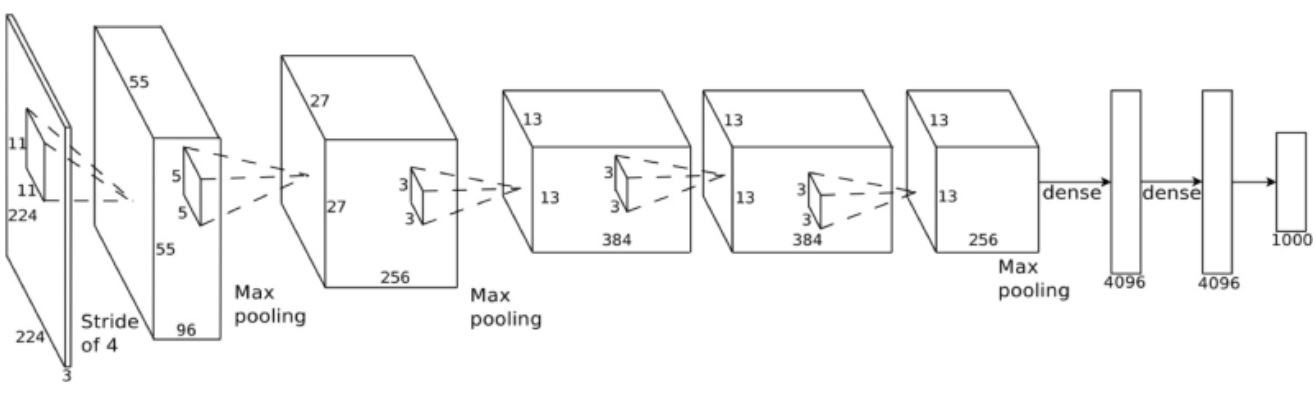
\includegraphics[width=0.6\textwidth]{img/cnn/cnn_architecture.jpg}
\end{tabular}
\end{figure}
\large{Every layer has a simple API: \emph{it transforms an input 3D volume to an output 3D volume with some differentiable function that may or may not have parameters}}.
\end{frame}

%%%%%%%%%%%%%%%%%%%%%%%%%%%%%%%%%%%%%%%%%%%%%%%%%%%%%%%%%%%%%%%%%%

\begin{frame}{Convolutional Layers}
The \textbf{Convolutional Layer} is the core building block of convolutional neural networks.\\
\vspace{0.2cm}
\textbf{Intuition}: every convolutional layer is equipped with a set of learnable filters. During the forward pass, each filter is convolved with the input volume thus producing a 2D activation map. One map for each filter is produced. The output volume is then made up by stacking all activation maps produced one on the top of the other. 	
\begin{figure}
\begin{tabular}{c}
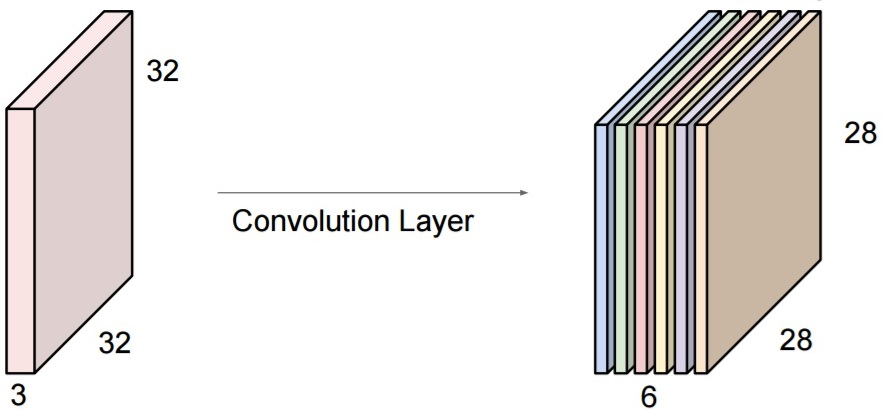
\includegraphics[width=0.4\textwidth]{img/cnn/activation_maps.jpg}\\
\small{\emph{e.g.} Result of $N=6$ filters of kernel size $K=5$x$5$ convolved on input image.}
\end{tabular}
\end{figure}
\end{frame}

%%%%%%%%%%%%%%%%%%%%%%%%%%%%%%%%%%%%%%%%%%%%%%%%%%%%%%%%%%%%%%%%%%
%%%%%%%%%%%%%%%%%%%%%%%%%%%%%%%%%%%%%%%%%%%%%%%%%%%%%%%%%%%%%%%%%%
%%%%%%%%%%%%%%%%%%%%%%%%%%%%%%%%%%%%%%%%%%%%%%%%%%%%%%%%%%%%%%%%%%


\section*{Convolutional Layers}

%%%%%%%%%%%%%%%%%%%%%%%%%%%%%%%%%%%%%%%%%%%%%%%%%%%%%%%%%%%%%%%%%%

\begin{frame}{Convolutional Layers}
Each convolutional layer has three main hyperparameters:
\begin{itemize}
\item Number of filters $N$
\item Kernel size $K$, the spatial size of the filters convolved
\item Filter stride $S$, factor by which to downscale
\end{itemize}
The presence and amount of spatial padding $P$ on the input volume may be considered an additional hyperparameter. In practice padding is usually performed to avoid headaches caused by convolutions "eating the borders".
\end{frame}

%%%%%%%%%%%%%%%%%%%%%%%%%%%%%%%%%%%%%%%%%%%%%%%%%%%%%%%%%%%%%%%%%%

\begin{frame}{Visualizing Convolution 2D}
\begin{figure}
\begin{tabular}{c}
Convolution 2D, half padding, stride $S=1$.\\
  \animategraphics[loop,controls,width=0.35\textwidth]{1}{img/cnn/conv_animation/conv_animation-}{0}{24}
\end{tabular}
\end{figure}
\end{frame}

%%%%%%%%%%%%%%%%%%%%%%%%%%%%%%%%%%%%%%%%%%%%%%%%%%%%%%%%%%%%%%%%%%

\begin{frame}{Visualizing Convolution 2D}
\begin{figure}
\begin{tabular}{c}
Convolution 2D, no padding, stride $S=2$.\\
  \animategraphics[loop,controls,width=0.35\textwidth]{1}{img/cnn/conv_animation_stride/conv_animation_stride-}{0}{3}
\end{tabular}
\end{figure}
\end{frame}

%%%%%%%%%%%%%%%%%%%%%%%%%%%%%%%%%%%%%%%%%%%%%%%%%%%%%%%%%%%%%%%%%%

\begin{frame}{Convolutional Layers: Local Connectivity}
Looking closer, neurons in a CNN perform the very same operation of the neurons we already know from DNN.
\begin{equation*}
		\sum_i w_i x_i + b
\end{equation*}
\begin{columns}
    \begin{column}{0.48\textwidth}
    \centering
		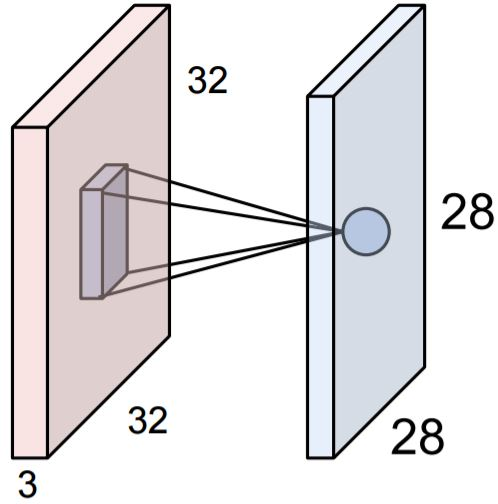
\includegraphics[width=0.5\textwidth]{img/cnn/local_connectivity.jpg}
    \end{column}
     \begin{column}{0.48\textwidth}
However, in convolutional layers neurons are only locally connected to the input volume. The small region that each neuron "sees" of the previous layer is usually referred to as the \textbf{receptive field} of the neuron.
    \end{column}
\end{columns}
\end{frame}

%%%%%%%%%%%%%%%%%%%%%%%%%%%%%%%%%%%%%%%%%%%%%%%%%%%%%%%%%%%%%%%%%%

\begin{frame}{Convolutional Layers: Parameter Sharing}
Assumption: if a feature is useful to compute at some spatial location $(x,y)$, then it should be useful to compute also at different locations $(x_i,y_i)$. \textbf{Thus, we constrain the neurons in each depth slice to use the same weights and bias.}

If all neurons in a single depth slice are using the same weight vector, then the forward pass of the convolutional layer can \emph{in each depth slice} be computed as a convolution of the neuron's weights with the input volume (hence the name). This is why it is common to refer to each set of weights as a filter (or a kernel), that is convolved with the input.
\end{frame}

%%%%%%%%%%%%%%%%%%%%%%%%%%%%%%%%%%%%%%%%%%%%%%%%%%%%%%%%%%%%%%%%%%

\begin{frame}{Convolutional Layers: Parameter Sharing}
\begin{figure}
\begin{tabular}{c}
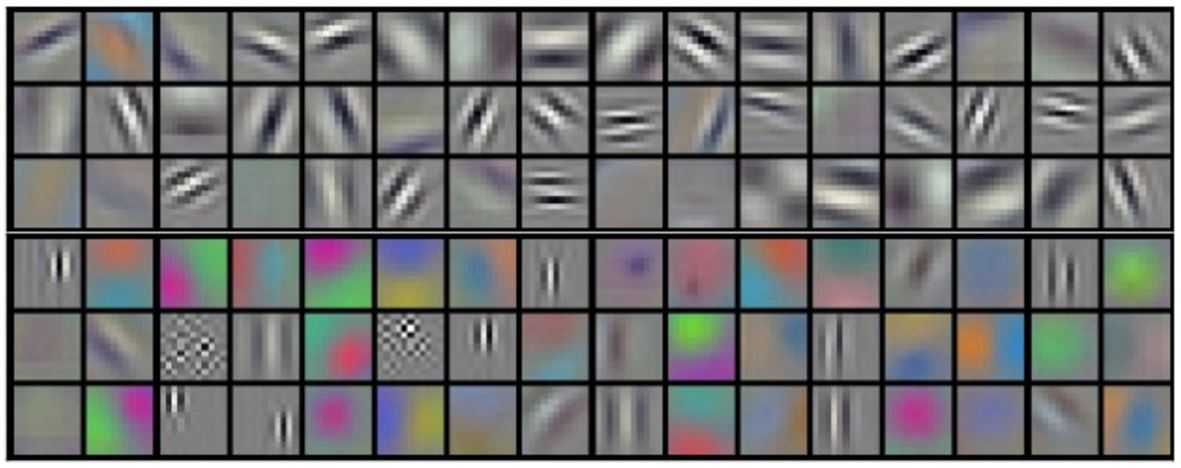
\includegraphics[width=0.80\textwidth]{img/cnn/learned_weights.jpg}
\end{tabular}
\end{figure}
\small{Example of weights learned by \cite{krizhevsky2012imagenet}. Each of the 96 filters shown here is of size [11x11x3], and each one is shared by the 55*55 neurons in one depth slice. Notice that the parameter sharing assumption is relatively reasonable: If detecting a horizontal edge is important at some location in the image, it should intuitively be useful at some other location as well due to the translationally-invariant structure of images.}
\end{frame}

%%%%%%%%%%%%%%%%%%%%%%%%%%%%%%%%%%%%%%%%%%%%%%%%%%%%%%%%%%%%%%%%%%

\begin{frame}{Convolutional Layers: Number of Learnable Parameters}
Given an input volume of size $H_1$ x $W_1$ x $C_1$, the number of \textbf{learnable parameters} of a convolutional layer with $N$ filters and kernel size $K$x$K$ is:
\begin{equation*}
tot\_learnable = N * K * K * C_1 + N
\end{equation*}
\small{\textit{Explanation}: there are N filters which convolve on input volume. The neural connection is local on width and height, but extends for the full depth of input volume, so there are $K * K * C_1$ parameters for each filter. Furthermore, each filter has an additive learnable bias.}
\end{frame}

%%%%%%%%%%%%%%%%%%%%%%%%%%%%%%%%%%%%%%%%%%%%%%%%%%%%%%%%%%%%%%%%%%
%%%%%%%%%%%%%%%%%%%%%%%%%%%%%%%%%%%%%%%%%%%%%%%%%%%%%%%%%%%%%%%%%%
%%%%%%%%%%%%%%%%%%%%%%%%%%%%%%%%%%%%%%%%%%%%%%%%%%%%%%%%%%%%%%%%%%


\section*{Pooling Layers}

\begin{frame}{Pooling Layers: overview}
Pooling layers spatially subsample the input volume.\\
Each depth slice of the input is processed independently.\\
\begin{figure}
\begin{tabular}{c}
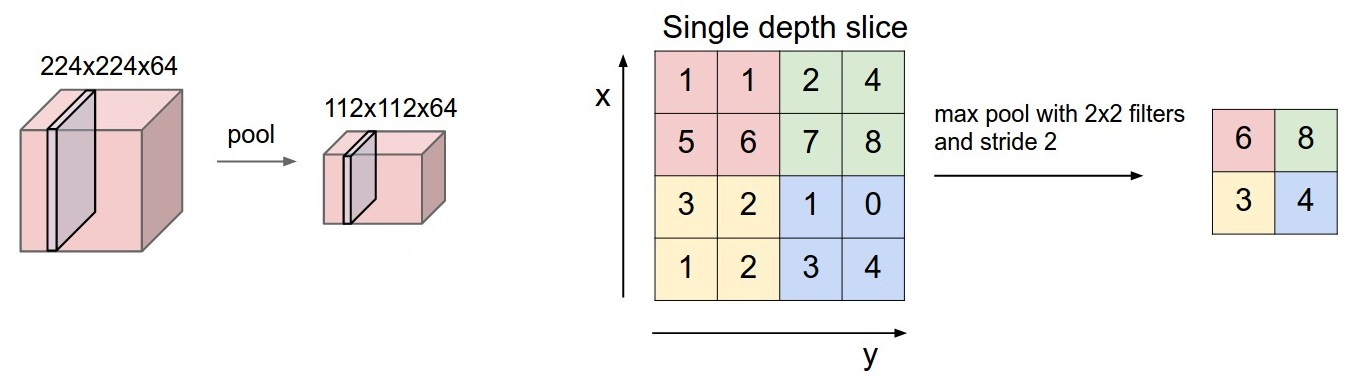
\includegraphics[width=0.90\textwidth]{img/cnn/pool.jpg}
\end{tabular}
\end{figure}
Two hyperparameters:
\begin{itemize}
\item Pool size $K$, which is the size of the pooling window
\item Pool stride $S$, which is the factor by which to downscale
\end{itemize}
%\begin{equation*}
%A_{i,j} = e^{-\frac{\sum_{k=1}^d||x_i^k-x_j^k||^2}{\sigma^2}}
%\end{equation*}
\end{frame}

%%%%%%%%%%%%%%%%%%%%%%%%%%%%%%%%%%%%%%%%%%%%%%%%%%%%%%%%%%%%%%%%%%

\begin{frame}{Pooling Layers: types}
The pooling function may be considered an additional hyperparameter.

In principle, many different functions could be used.

In practice, the \textbf{max} pooling is by far the most common
\begin{equation*}
h^n_i(x, y) = max_{\bar{x},\bar{y} \in N(x, y)}h^{n-1}_{i}(\bar{x},\bar{y})
\end{equation*}
Another common pooling function is the \textbf{average}
\begin{equation*}
h^n_i(x, y) = \frac{1}{K}\sum_{\bar{x},\bar{y} \in N(x, y)}h^{n-1}_{i}(\bar{x},\bar{y})
\end{equation*}
\end{frame}

%%%%%%%%%%%%%%%%%%%%%%%%%%%%%%%%%%%%%%%%%%%%%%%%%%%%%%%%%%%%%%%%%%

\begin{frame}{Pooling Layers: why}
Pooling layers are widely used for a number of reasons:
\begin{itemize}
\item Gain robustness to exact location of the features
\item Reduce computational (memory) cost
\item Help preventing overfitting
\item Increase receptive field of following layers
\end{itemize}
Most common configuration: pool size $K=2$x$2$, stride $S=2$. In this setting 75\% of input volume activations are discarded.
\end{frame}

%%%%%%%%%%%%%%%%%%%%%%%%%%%%%%%%%%%%%%%%%%%%%%%%%%%%%%%%%%%%%%%%%%

\begin{frame}{Pooling Layers: why not}
\textbf{The loss of spatial resolution is not always beneficial}.\\
\emph{e.g.} semantic segmentation
\begin{figure}
\begin{tabular}{cc}
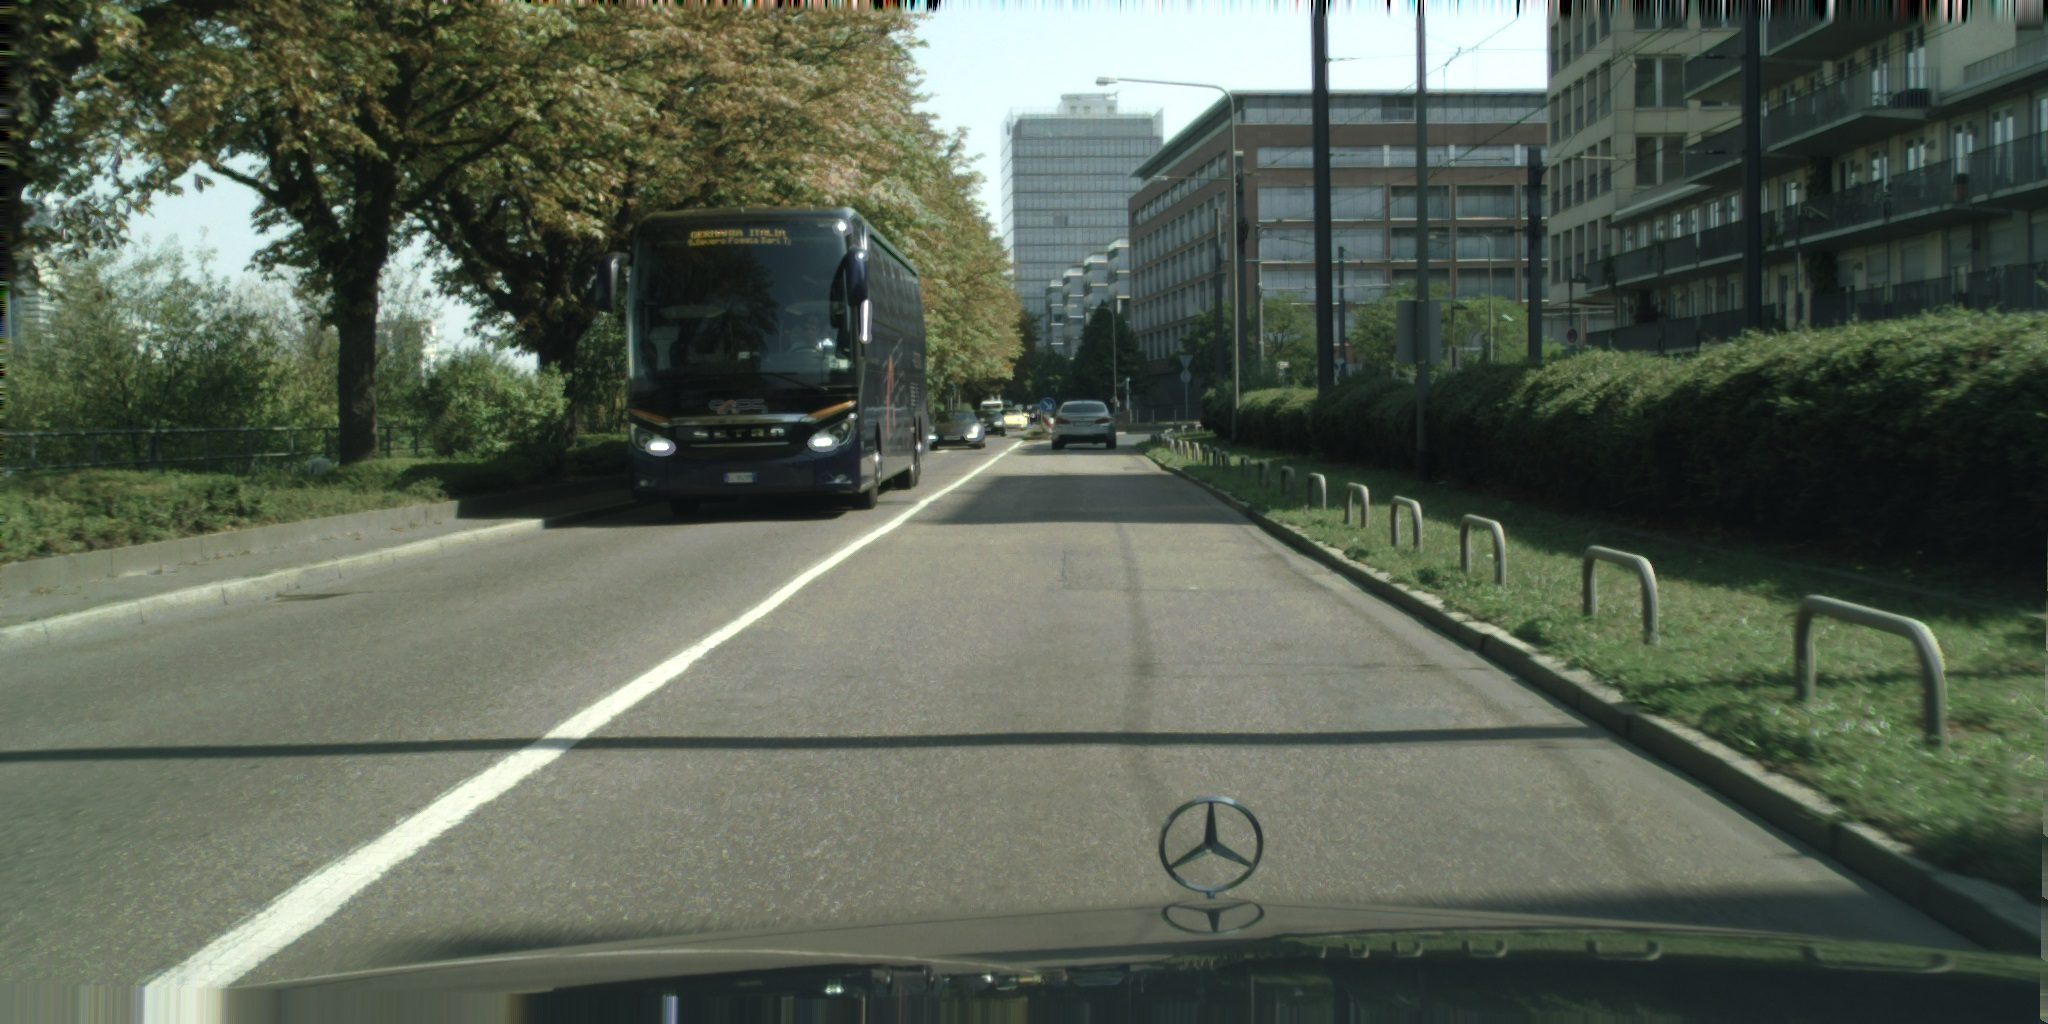
\includegraphics[width=0.4\textwidth]{img/cnn/semseg_in.jpg}&
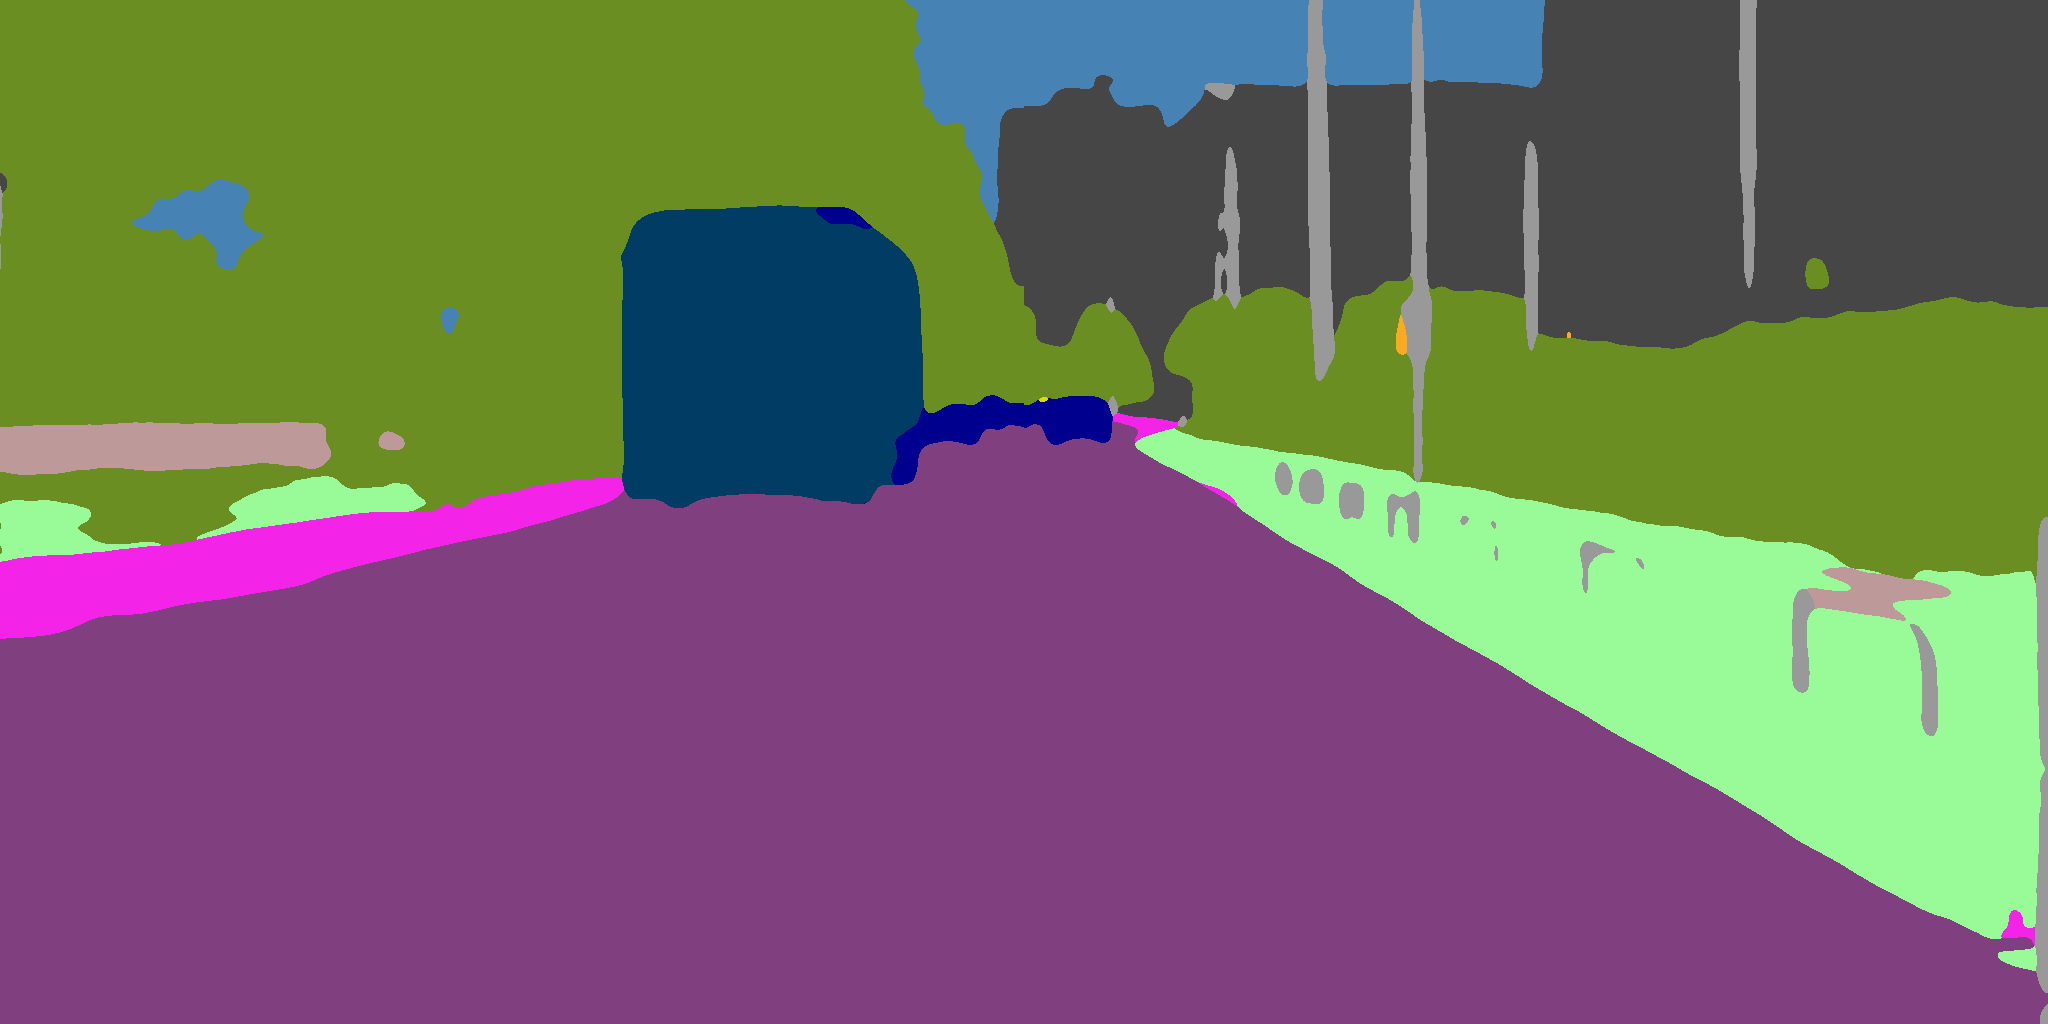
\includegraphics[width=0.4\textwidth]{img/cnn/semseg_out.png}
\end{tabular}
\end{figure}
There's a lot of research on getting rid of pooling layers while mantaining the benefits (\emph{e.g.} \cite{springenberg2014striving,yu2015multi}). We'll see if future architecture will still feature pooling layers.
\end{frame}

%%%%%%%%%%%%%%%%%%%%%%%%%%%%%%%%%%%%%%%%%%%%%%%%%%%%%%%%%%%%%%%%%%
%%%%%%%%%%%%%%%%%%%%%%%%%%%%%%%%%%%%%%%%%%%%%%%%%%%%%%%%%%%%%%%%%%
%%%%%%%%%%%%%%%%%%%%%%%%%%%%%%%%%%%%%%%%%%%%%%%%%%%%%%%%%%%%%%%%%%

\section*{Activation Layers}

\begin{frame}{Activation Layers}

Activation layers compute non-linear activation function elementwise on the input volume. The most common activations are \textbf{ReLu}, \textbf{sigmoid} and \textbf{tanh}.
\begin{figure}
\begin{tabular}{ccc}
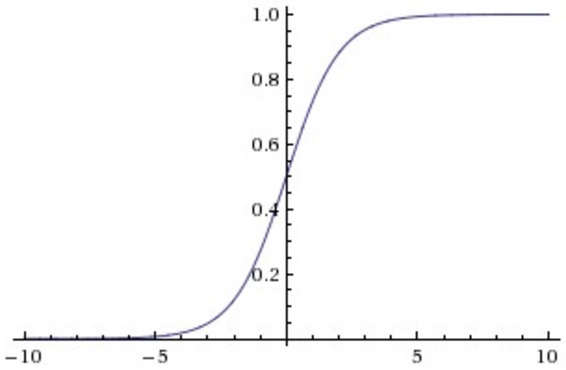
\includegraphics[width=0.3\textwidth]{img/cnn/act_sigmoid.jpg}&
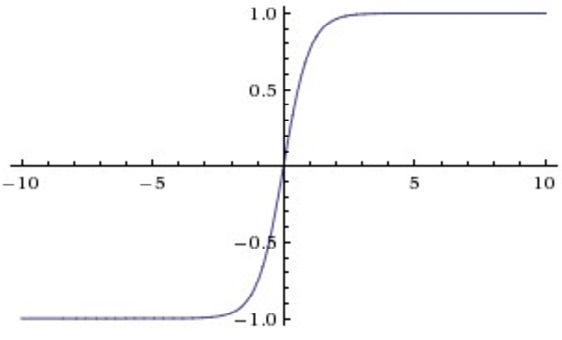
\includegraphics[width=0.3\textwidth]{img/cnn/act_tanh.jpg} & 
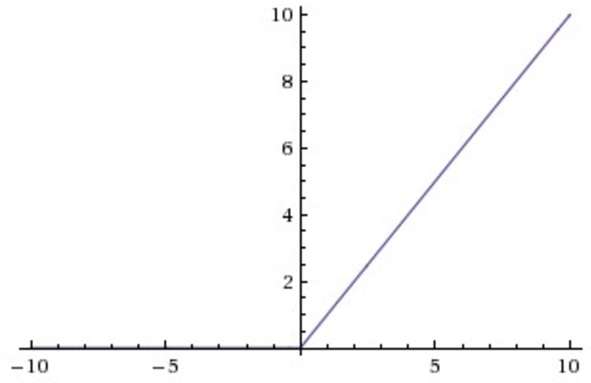
\includegraphics[width=0.3\textwidth]{img/cnn/act_relu.jpg}\\
Sigmoid & Tanh & ReLu
\end{tabular}
\end{figure}
Nonetheless, more complex activation functions exist \cite{he2015delving,goodfellow2013maxout}.
\end{frame}

%%%%%%%%%%%%%%%%%%%%%%%%%%%%%%%%%%%%%%%%%%%%%%%%%%%%%%%%%%%%%%%%%%

\begin{frame}{Activation Layers}
\textbf{ReLu wins}\\
ReLu was found to greatly accelerate the convergence of SGD compared to sigmoid/tanh functions \cite{krizhevsky2012imagenet}. Furthermore, ReLu can be implemented by a simple threshold, \emph{w.r.t.} other activations which require complex operations.

\textbf{Why using non-linear activations at all?}\\
Composition of linear functions is a linear function. Without nonlinearities, neural networks would reduce to 1 layer logistic regression.\\

\end{frame}

%%%%%%%%%%%%%%%%%%%%%%%%%%%%%%%%%%%%%%%%%%%%%%%%%%%%%%%%%%%%%%%%%%

\begin{frame}{Computing Output Volume Size}
\textbf{Convolutional layer}: given an input volume of size $H_1$ x $W_1$ x $C_1$, the output of a convolutional layer with $N$ filters, kernel size $K$, stride $S$ and zero padding $P$ is a volume with new shape $H_2$ x $W_2$ x $C_2$, where:
\begin{itemize}
\item $H_2 = (H_1 - K + 2P) / S + 1$ 
\item $W_2 = (W_1 - K + 2P) / S + 1$ 
\item $C_2 = N$
\end{itemize}
\end{frame}

%%%%%%%%%%%%%%%%%%%%%%%%%%%%%%%%%%%%%%%%%%%%%%%%%%%%%%%%%%%%%%%%%%

\begin{frame}{Computing Output Volume Size}
\textbf{Pooling layer}: given an input volume of size $H_1$ x $W_1$ x $C_1$, the output of a pooling layer with pool size $K$ and pool stride $S$ is a volume with new shape $H_2$ x $W_2$ x $C_2$, where:
\begin{itemize}
\item $H_2 = (H_1 - K) / S + 1$ 
\item $W_2 = (W_1 - K) / S + 1$ 
\item $C_2 = C_1$
\end{itemize}
\textbf{Activation layer}: given an input volume of size $H_1$ x $W_1$ x $C_1$, the output of an activation layer is a volume with shape $H_2$ x $W_2$ x $C_2$, where:
\begin{itemize}
\item $H_2 = H_1$ 
\item $W_2 = W_1$ 
\item $C_2 = C_1$
\end{itemize}
\end{frame}

%%%%%%%%%%%%%%%%%%%%%%%%%%%%%%%%%%%%%%%%%%%%%%%%%%%%%%%%%%%%%%%%%%

\begin{frame}{Advanced CNN Architectures}
More complex CNN architectures have recently been demonstrated to perform better than the traditional \texttt{conv -> relu -> pool } stack architecture.

These architectures usually feature different graph topologies and much more intricate connectivity structures (\emph{e.g.} \cite{he2016deep,szegedy2016rethinking}).

However, these advanced architectures are out of the scope of these lectures.
\end{frame}

%%%%%%%%%%%%%%%%%%%%%%%%%%%%%%%%%%%%%%%%%%%%%%%%%%%%%%%%%%%%%%%%%%
%%%%%%%%%%%%%%%%%%%%%%%%%%%%%%%%%%%%%%%%%%%%%%%%%%%%%%%%%%%%%%%%%%
%%%%%%%%%%%%%%%%%%%%%%%%%%%%%%%%%%%%%%%%%%%%%%%%%%%%%%%%%%%%%%%%%%

\section{Case Study: VGG Network}

\begin{frame}{VGG}
\textbf{VGG} \cite{simonyan2014very} indicates a deep convolutional network for image recognition developed and trained in 2014 by the Oxford Vision Geometry Group.\\
\vspace{0.25cm}
This network is well-known for a variety of reasons:
\begin{itemize}
\item \textbf{Performance} of the network is (was) great. In 2014 VGG team secured the first and the second places in the localization and classification challenge on ImageNet;
\item \textbf{Pre-trained weights were released} in Caffe \cite{jia2014caffe} and converted by the deep learning community in a variety of other frameworks;
\item \textbf{Architectural choices} by the authors led to a very neat network model, successively taken as guideline for a number of future works.
\end{itemize} 
\end{frame}

%%%%%%%%%%%%%%%%%%%%%%%%%%%%%%%%%%%%%%%%%%%%%%%%%%%%%%%%%%%%%%%%%%

\begin{frame}{VGG16 Architecture}
\vspace{-0.5cm}
\begin{columns}
	\begin{column}{0.1\textwidth}
		\begin{figure}
			\begin{tabular}{c}
				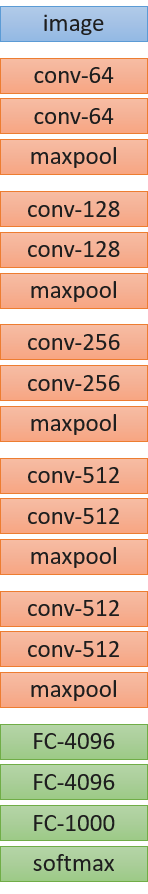
\includegraphics[width=0.8\textwidth]{img/cnn/vgg16_architecture.png}
			\end{tabular}
		\end{figure}
	\end{column}
	\begin{column}{0.9\textwidth}
		\\ \vspace{0.5cm}
		\textbf{Input} fixed size 224x224 RGB images. For training, images are pre-processed subtracting the mean RGB value of the training set.\\
		\vspace{0.25cm}
		\textbf{Convolutional filters} feature 3x3 receptive field (the smallest size to capture the notion of left/right, up/down, center) and stride is fixed to 1 pixel.\\
		\vspace{0.25cm}
		\textbf{Spatial pooling} is carried out by five max pooling layers performed over 2x2 pixel window, with stride 2.\\
		\vspace{0.25cm}
		\textbf{ReLu activation} follow all hidden layers.\\
		\vspace{0.25cm}
		\textbf{Fully connected} layers feature 4096 neurons each followed by ReLu. The very last fully connected layer is composed of 1000 neurons (as many as ImageNet classes) and is followed by softmax activation.
	\end{column}
\end{columns}
\end{frame}

%%%%%%%%%%%%%%%%%%%%%%%%%%%%%%%%%%%%%%%%%%%%%%%%%%%%%%%%%%%%%%%%%%

\begin{frame}{VGG16 Computational Footprint}
\vspace{-0.5cm}
\begin{columns}
	\begin{column}{0.1\textwidth}
		\begin{figure}
			\begin{tabular}{c}
				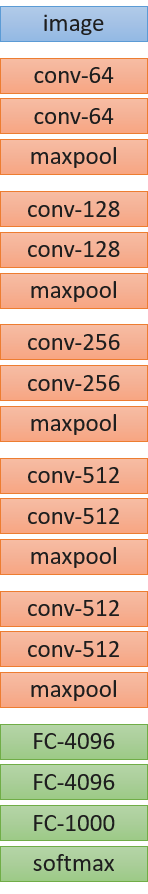
\includegraphics[width=0.8\textwidth]{img/cnn/vgg16_architecture.png}
			\end{tabular}
		\end{figure}
	\end{column}
	\begin{column}{0.9\textwidth}
		VGG16 features a total of \textbf{138 M learnable parameters}.\\
		\vspace{0.5cm}
		\textbf{Each image takes approx. 93MB of memory for forward pass}. As a rule of thumb, backward pass consumes roughly the double of the resources. Most of memory usage is due to the first layers in the network.\\
		\vspace{0.5cm}
		\textbf{Most of learnable parameters (70\%) are condensed in the last fully-connected layers}. In particular, one single layer is responsible of approximately 100M parameters on the total of 138M (can you spot it?). 
	\end{column}
\end{columns}
\end{frame}

%%%%%%%%%%%%%%%%%%%%%%%%%%%%%%%%%%%%%%%%%%%%%%%%%%%%%%%%%%%%%%%%%%
%%%%%%%%%%%%%%%%%%%%%%%%%%%%%%%%%%%%%%%%%%%%%%%%%%%%%%%%%%%%%%%%%%
%%%%%%%%%%%%%%%%%%%%%%%%%%%%%%%%%%%%%%%%%%%%%%%%%%%%%%%%%%%%%%%%%%

\section{Visualizing what CNNs Learn}

\begin{frame}{The Myth of Interpretability}
Convolutional neural networks have often been \textbf{criticized for their lack of interpretability}\cite{lipton2016mythos}. The main objection is to deal with big and complex black boxes, that give correct results even if in which we have no cue of what's happening inside.\\
\vspace{-0.25cm}
\begin{figure}
\begin{tabular}{c}
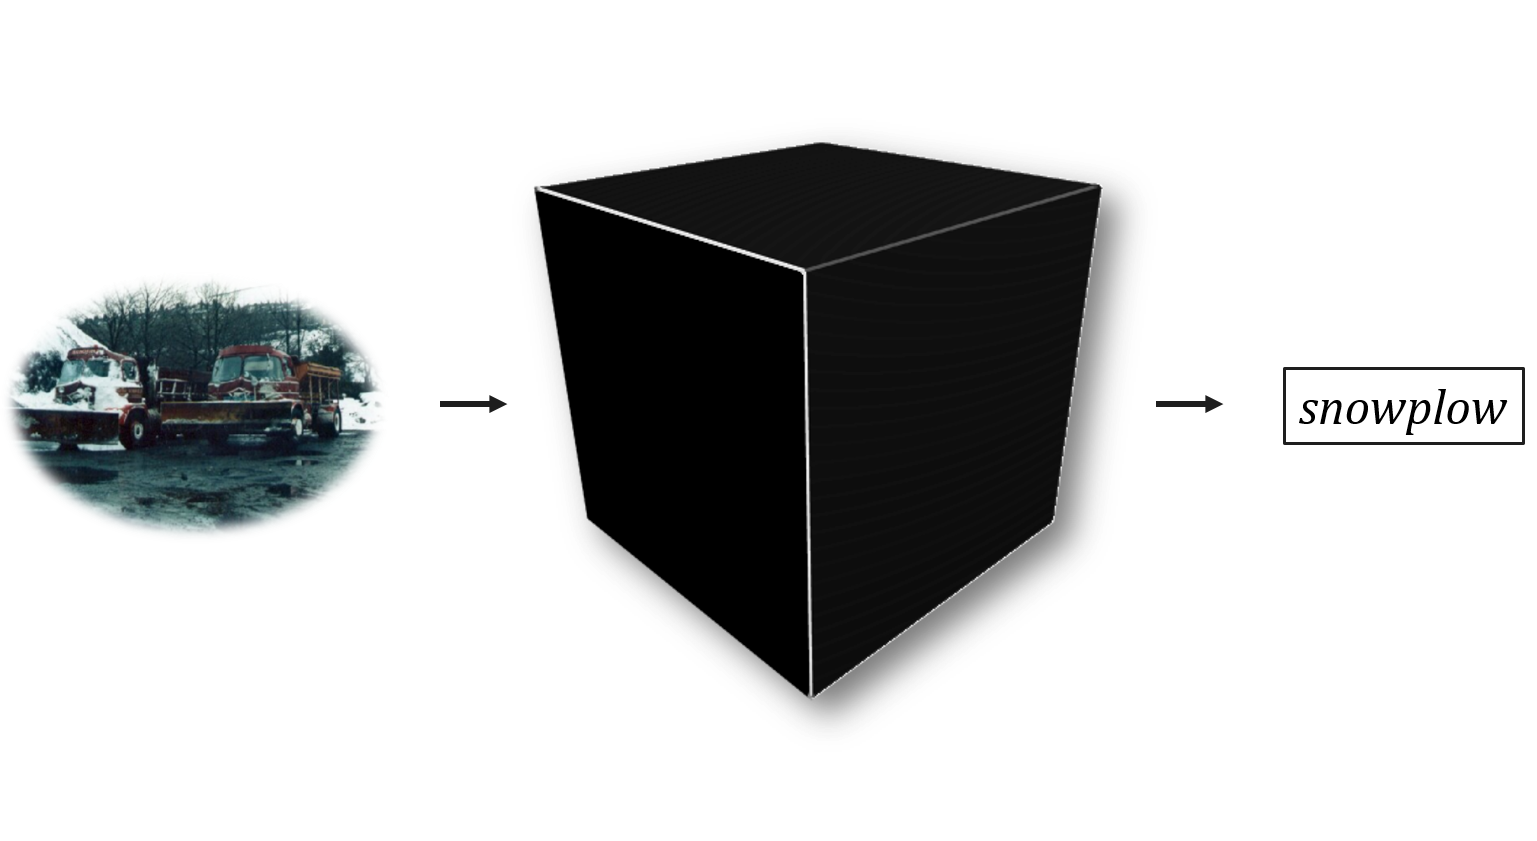
\includegraphics[width=0.75\textwidth]{img/cnn/black_box.png}
\end{tabular}
\end{figure}
\end{frame}

%%%%%%%%%%%%%%%%%%%%%%%%%%%%%%%%%%%%%%%%%%%%%%%%%%%%%%%%%%%%%%%%%%

\begin{frame}{The Myth of Interpretability}
On the other side, \textbf{linear models} and \textbf{decision trees} are often presented as example of "champions" of interpretability. The debate whether a logistic regression would be more or less interpretable than a deep network is complex out the scope of this lecture.\\
\vspace{0.5cm}
Partly as a response to this criticism, \textbf{several methods have been developed in literature to visualize what a CNN learned}. Let's see some examples.
\end{frame}

%%%%%%%%%%%%%%%%%%%%%%%%%%%%%%%%%%%%%%%%%%%%%%%%%%%%%%%%%%%%%%%%%%

\begin{frame}{Visualizing Activations}
\textbf{Visualizing activations} of the network during the forward pass is straightforward and can be useful to detect dead filters (i.e. activations that are zero whatever the input).% Usually activations start looking relatively dense and become more sparse and localized as the training progresses.
\begin{figure}
\begin{tabular}{c}
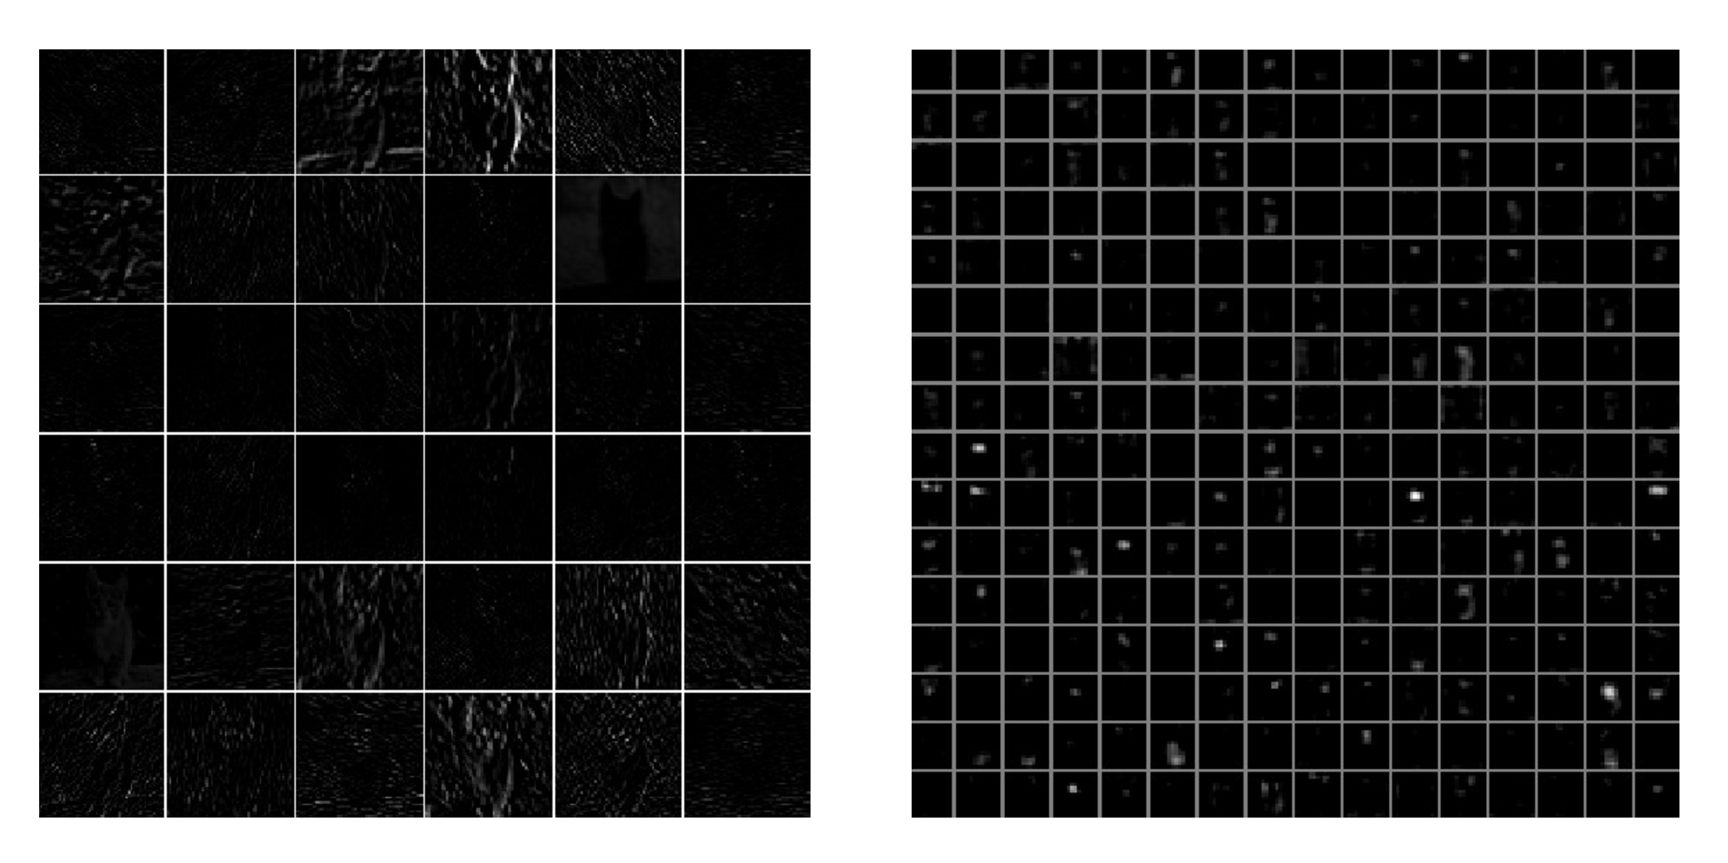
\includegraphics[width=0.6\textwidth]{img/cnn/visualize_activation.png} 
\end{tabular}
\caption{Activations on the 1st \texttt{conv} layer (left), and the 5th \texttt{conv} layer (right) of a trained AlexNet looking at a picture of a cat. Every box shows an activation map corresponding to some filter. Notice that the activations are sparse and mostly local.}
\end{figure}
\end{frame}

%%%%%%%%%%%%%%%%%%%%%%%%%%%%%%%%%%%%%%%%%%%%%%%%%%%%%%%%%%%%%%%%%%

\begin{frame}{Inspecting Weights}
\textbf{Visualizing the learned weights} is another common strategy to get an insight of what the network looks for in the images. The most interpretable weights are the ones learned by first convolutional layer, which operates directly on the image pixels.
\begin{figure}
\begin{tabular}{c}
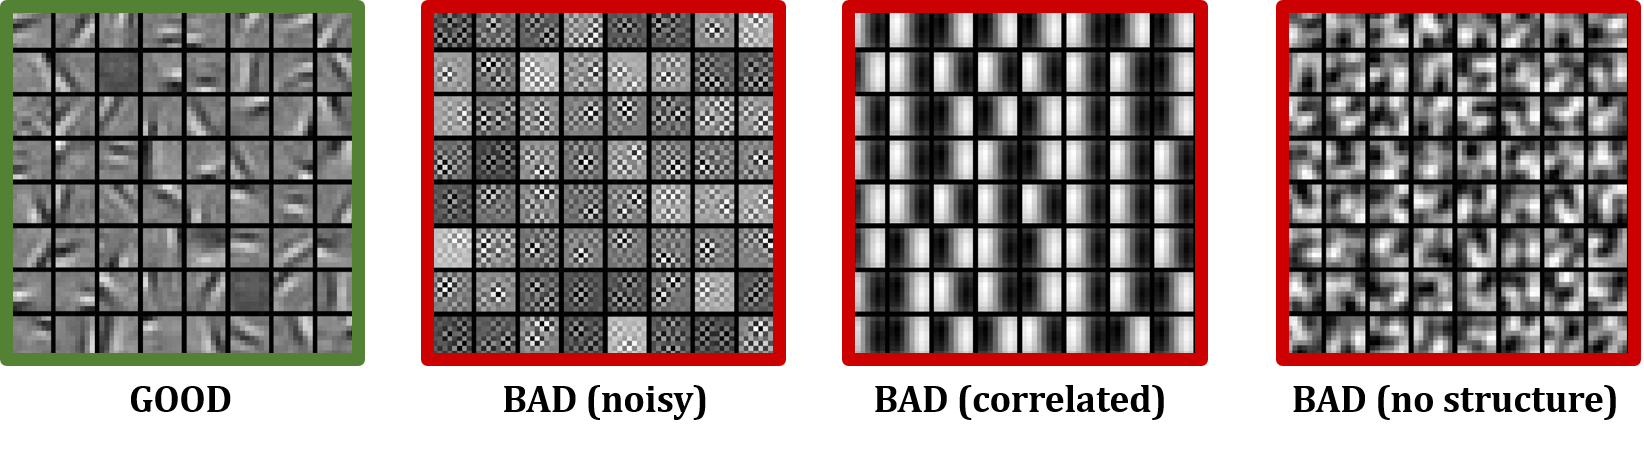
\includegraphics[width=\textwidth]{img/cnn/weights_inspection.png}
\end{tabular}
\end{figure}

\end{frame}

%%%%%%%%%%%%%%%%%%%%%%%%%%%%%%%%%%%%%%%%%%%%%%%%%%%%%%%%%%%%%%%%%%

\begin{frame}{Partially Occluding the Images}
To investigate which portion of the input image most contributed to a certain prediction, we can slide an occluding object on the input, and seeing how the class probability changes as a function of the position of the occluder object \cite{zeiler2014visualizing}.
\begin{figure}
\begin{tabular}{c}
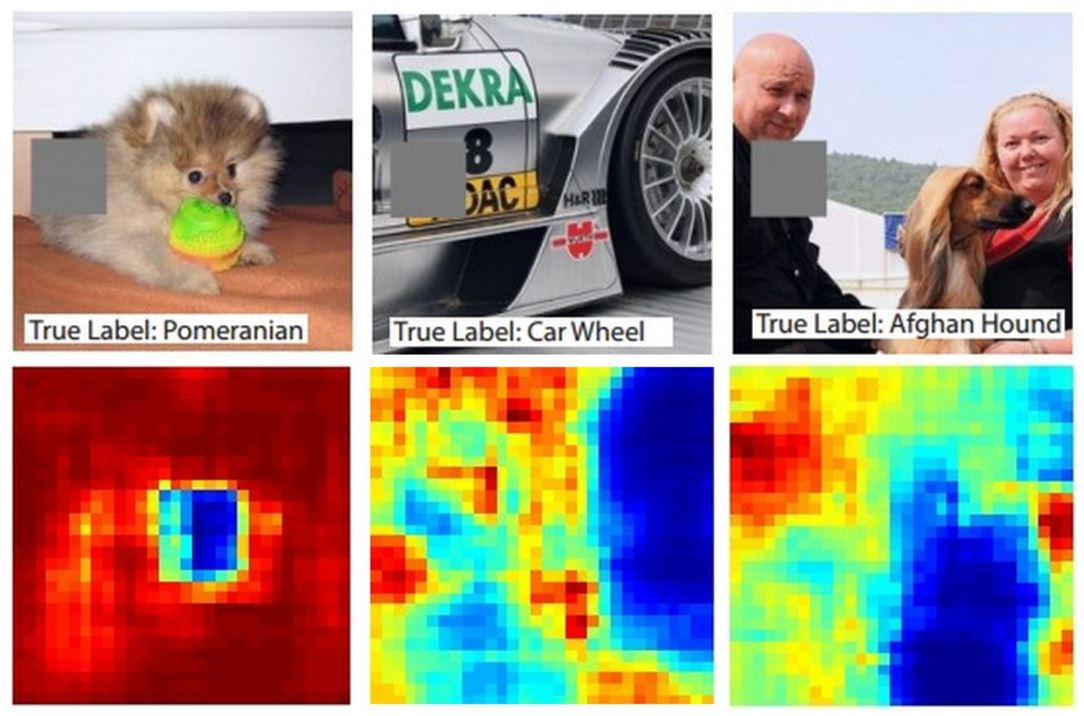
\includegraphics[width=0.5\textwidth]{img/cnn/occlusions.jpg}
\end{tabular}
\end{figure}
\end{frame}

%%%%%%%%%%%%%%%%%%%%%%%%%%%%%%%%%%%%%%%%%%%%%%%%%%%%%%%%%%%%%%%%%%

\begin{frame}{t-SNE Embedding}
CNNs can be interpreted as gradually transforming the images into a representation in which the classes are separable by a linear classifier. We can get a rough idea about the topology of this space by embedding images into two dimensions so that their low-dimensional representation has approximately equal distances than their high-dimensional representation. Here, a \textbf{t-SNE embedding} of a set of images.
\begin{figure}
\begin{tabular}{c}
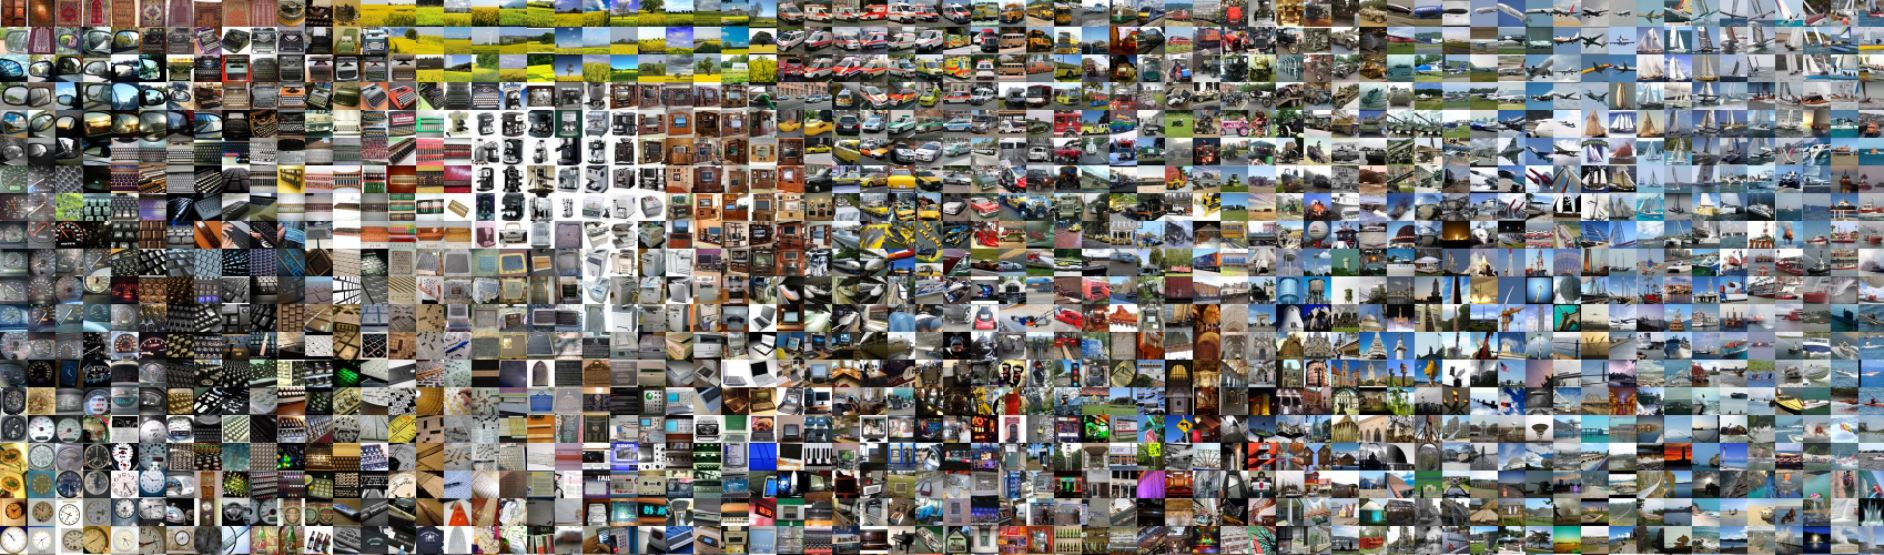
\includegraphics[width=0.8\textwidth]{img/cnn/tsne.jpg}
\end{tabular}
\end{figure}
\end{frame}

%%%%%%%%%%%%%%%%%%%%%%%%%%%%%%%%%%%%%%%%%%%%%%%%%%%%%%%%%%%%%%%%%%
%%%%%%%%%%%%%%%%%%%%%%%%%%%%%%%%%%%%%%%%%%%%%%%%%%%%%%%%%%%%%%%%%%
%%%%%%%%%%%%%%%%%%%%%%%%%%%%%%%%%%%%%%%%%%%%%%%%%%%%%%%%%%%%%%%%%%

\section{Transfer Learning}

%%%%%%%%%%%%%%%%%%%%%%%%%%%%%%%%%%%%%%%%%%%%%%%%%%%%%%%%%%%%%%%%%%

\begin{frame}{Transfer Learning}
\vspace{-1cm}
\begin{figure}
\begin{tabular}{c}
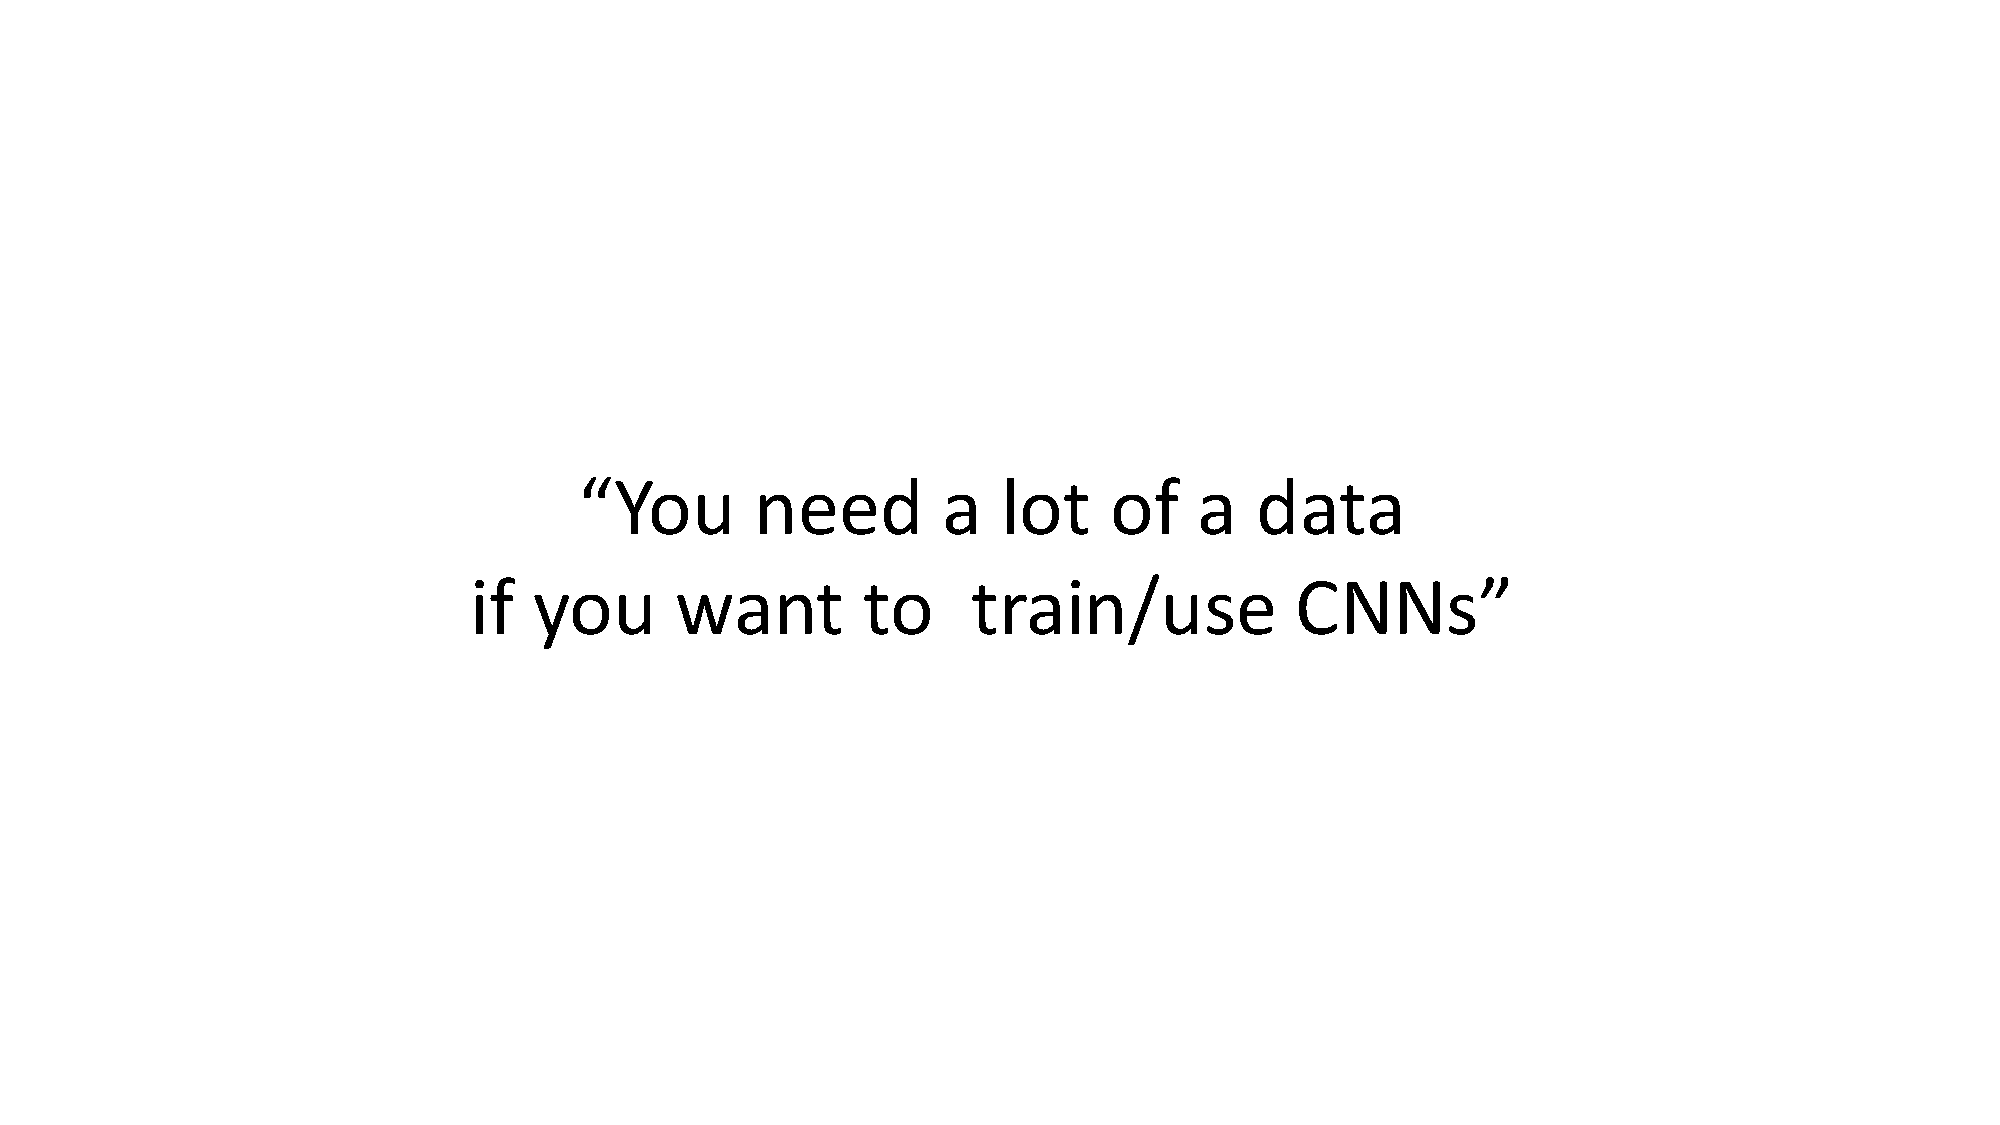
\includegraphics[width=\textwidth]{img/cnn/busted_0.pdf}
\end{tabular}
\end{figure}
\end{frame}

\begin{frame}{Transfer Learning}
\vspace{-1cm}
\begin{figure}
\begin{tabular}{c}

\includegraphics[width=\textwidth]{img/cnn/busted_1.pdf}
\end{tabular}
\end{figure}
\end{frame}

%%%%%%%%%%%%%%%%%%%%%%%%%%%%%%%%%%%%%%%%%%%%%%%%%%%%%%%%%%%%%%%%%%

\begin{frame}{Transfer Learning}
In practice, \textbf{for many applications there is no need to retrain an entire CNN from scratch}.\\
\vspace{0.5cm}
Conversely, few "famous" CNN architectures (e.g. VGG \cite{simonyan2014very}, ResNet \cite{he2016deep}) pretrained on ImageNet \cite{deng2009imagenet} are often used as initialization or feature extractor for a variety of tasks.
\end{frame}

%%%%%%%%%%%%%%%%%%%%%%%%%%%%%%%%%%%%%%%%%%%%%%%%%%%%%%%%%%%%%%%%%%\\

\begin{frame}{Transfer Learning}
\begin{figure}
\begin{tabular}{c}
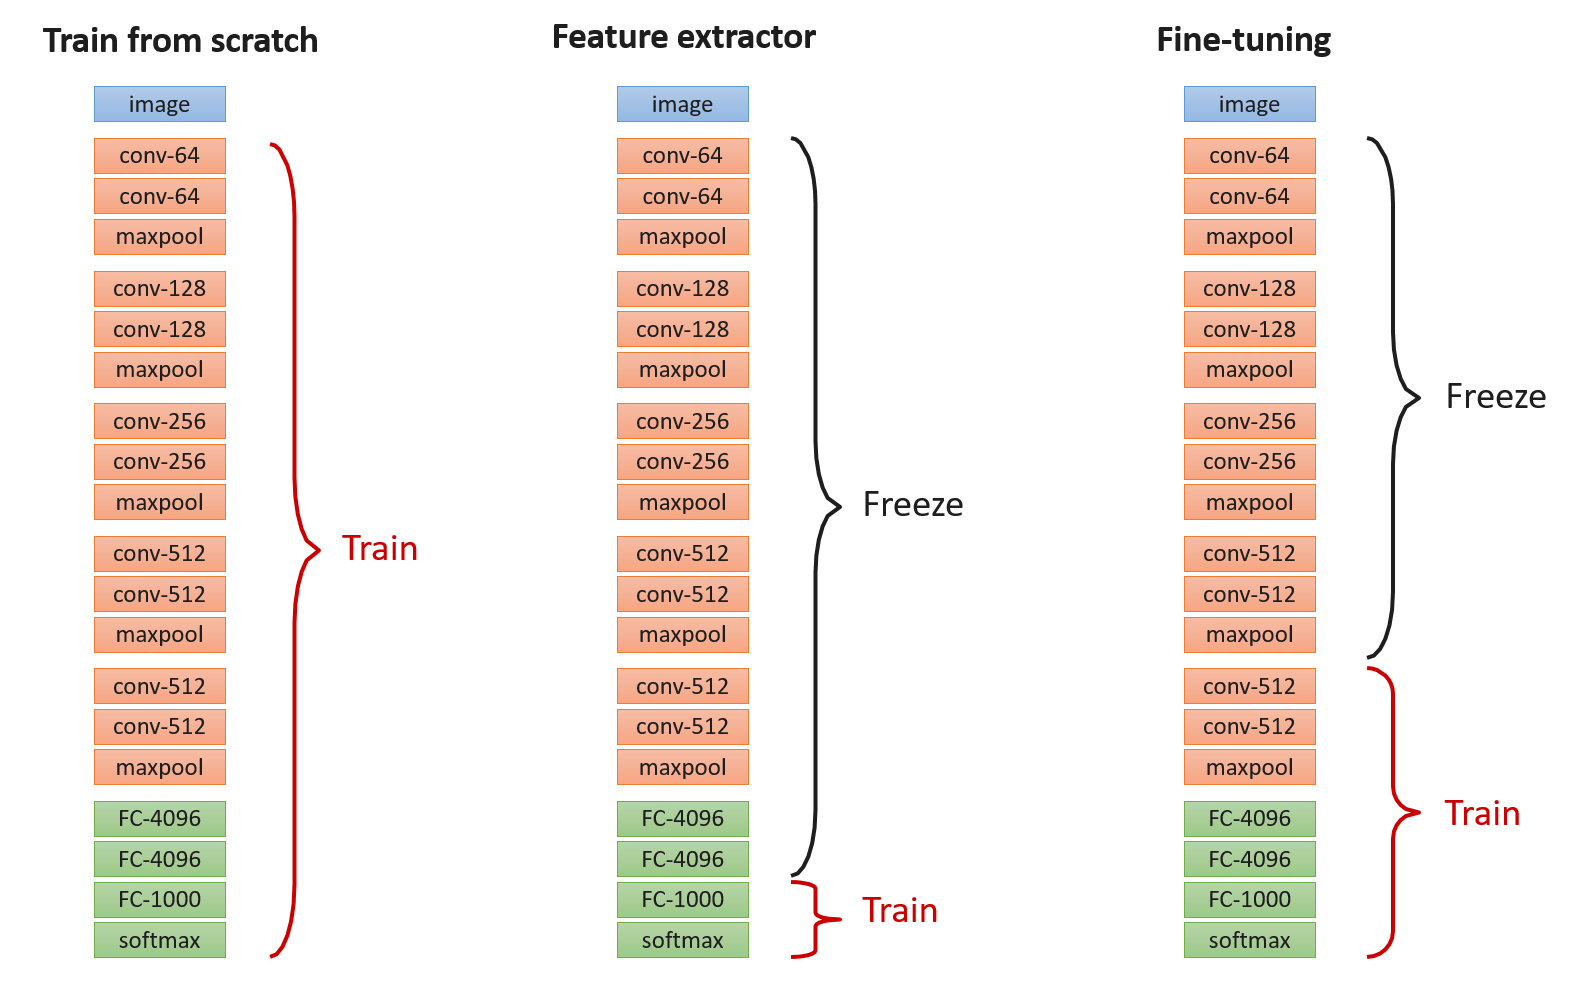
\includegraphics[width=0.7\textwidth]{img/cnn/training_possibilities.png}
\end{tabular}
\caption{Overview of three different training scenarios.}
\end{figure}
\end{frame}

%%%%%%%%%%%%%%%%%%%%%%%%%%%%%%%%%%%%%%%%%%%%%%%%%%%%%%%%%%%%%%%%%%

\begin{frame}{Transfer Learning}
Deciding which portion of the network must be retrained is a very important choice that will heavily influence the final model performance.\\
\vspace{0.5cm}
Generally speaking, two main factors influence this decision:
\begin{itemize}
\item \textbf{size of the new dataset}: if the new dataset is small, fine-tune big portion of the network is likely to lead to overfitting. The best choice might be to train a linear classifier of CNN features.
\item \textbf{similarity of the new data w.r.t. the original dataset}: the more similar is the new dataset w.r.t. the old one, the more we can confidently fine-tune the model without risking to overfit (given that we have enough data to do it).
\end{itemize}
\end{frame}

%%%%%%%%%%%%%%%%%%%%%%%%%%%%%%%%%%%%%%%%%%%%%%%%%%%%%%%%%%%%%%%%%%

\begin{frame}{Transfer Learning}
\begin{figure}
\begin{tabular}{c}
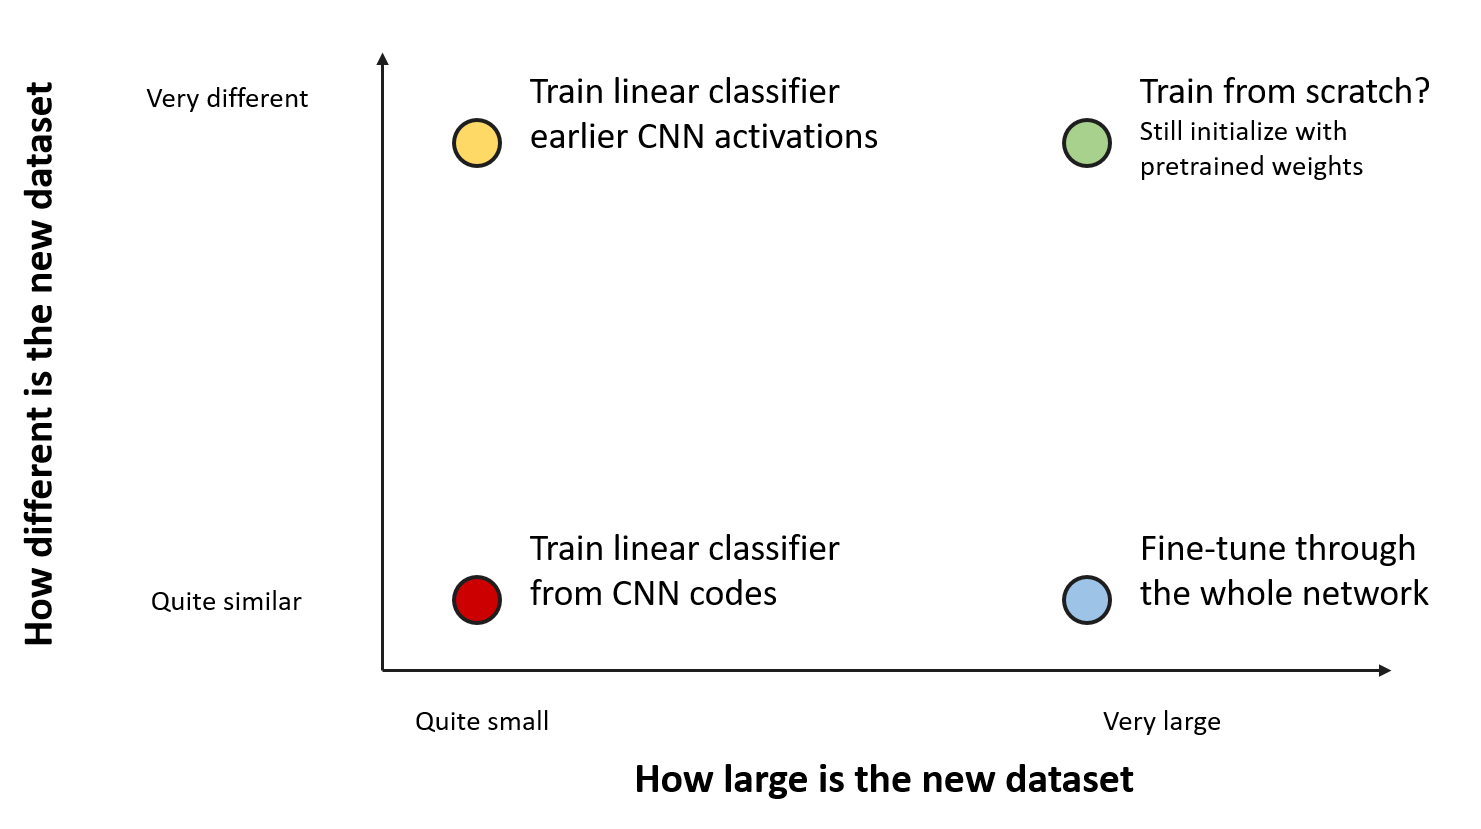
\includegraphics[width=0.8\textwidth]{img/cnn/finetuning_rules.png}
\end{tabular}
\caption{Rule of thumb for deciding how much of the model is to be retrained.}
\end{figure}
\end{frame}
%%%%%%%%%%%%%%%%%%%%%%%%%%%%%%%%%%%%%%%%%%%%%%%%%%%%%%%%%%%%%%%%%%

%\begin{frame}{Troubleshooting}
%\begin{itemize}
%\item Check gradient numerically by finite differences:
%\begin{equation*}
%f'(x) = \frac{f(x+\epsilon) - f(x-\epsilon)}{2\epsilon}
%\end{equation*}
%\end{itemize}
%\end{frame}

%%%%%%%%%%%%%%%%%%%%%%%%%%%%%%%%%%%%%%%%%%%%%%%%%%%%%%%%%%%%%%%%%%

%%%%%%%%%%%%%%%%%%%%%%%%%%%%%%%%%%%%%%%%%%%%%%%%%%%%%%%%%%%%%%%%%%
%%%%%%%%%%%%%%%%%%%%%%%%%%%%%%%%%%%%%%%%%%%%%%%%%%%%%%%%%%%%%%%%%%
%%%%%%%%%%%%%%%%%%%%%%%%%%%%%%%%%%%%%%%%%%%%%%%%%%%%%%%%%%%%%%%%%%

\section{Credits}
\begin{frame}[t, allowframebreaks]{Credits}
These slides heavily borrow from a number of awesome sources. I'm really grateful to all the people who take the time to share their knowledge on this subject with others.\\
\vspace{0.5cm}
In particular:
\begin{itemize}
\item Stanford CS231n Convolutional Neural Networks for Visual Recognition\\
\url{http://cs231n.stanford.edu/}
\item Stanford CS20SI TensorFlow for Deep Learning Research\\
\url{http://web.stanford.edu/class/cs20si/syllabus.html}
\item Deep Learning Book (GoodFellow, Bengio, Courville)\\
\url{http://www.deeplearningbook.org/}
\item Marc'Aurelio Ranzato, "Large-Scale Visual Recognition with Deep Learning"\\
\url{www.cs.toronto.edu/~ranzato/publications/ranzato_cvpr13.pdf}
\item Convolution arithmetic animations\\
\url{https://github.com/vdumoulin/conv_arithmetic}
\item Andrej Karphathy personal blog\\
\url{http://karpathy.github.io/}
\item WildML blog on AI, DL and NLP\\
\url{http://www.wildml.com/}
\item Michael Nielsen Deep Learning online book
\url{http://neuralnetworksanddeeplearning.com/}
\end{itemize}
\end{frame}

%%%%%%%%%%%%%%%%%%%%%%%%%%%%%%%%%%%%%%%%%%%%%%%%%%%%%%%%%%%%%%%%%%
%%%%%%%%%%%%%%%%%%%%%%%%%%%%%%%%%%%%%%%%%%%%%%%%%%%%%%%%%%%%%%%%%%
%%%%%%%%%%%%%%%%%%%%%%%%%%%%%%%%%%%%%%%%%%%%%%%%%%%%%%%%%%%%%%%%%%

\section{References}

\begin{frame}[t, allowframebreaks]
\frametitle{References}
\bibliographystyle{abbrv}
\bibliography{bibliography}
\end{frame}
\end{document}